\problem{}

\subproblem{}
کافیست یک مثال نقض از توزیعی بیاورم که میانگین آن (که برای توزیع پیوسته به صورت امید ریاضی تعریف میشود) جایی باشد که تابع توزیع آن برابر با یک دوم نشود. برای مثال در شکل زیر تنها نقطه ای که F(x) برای آن برابر با یک دوم میشود صفر است اما به وضوح امید ریاضی یا همان میانگین این نمودار بزرگ تر از صفر است.

\begin{figure}[H]
	\centering
	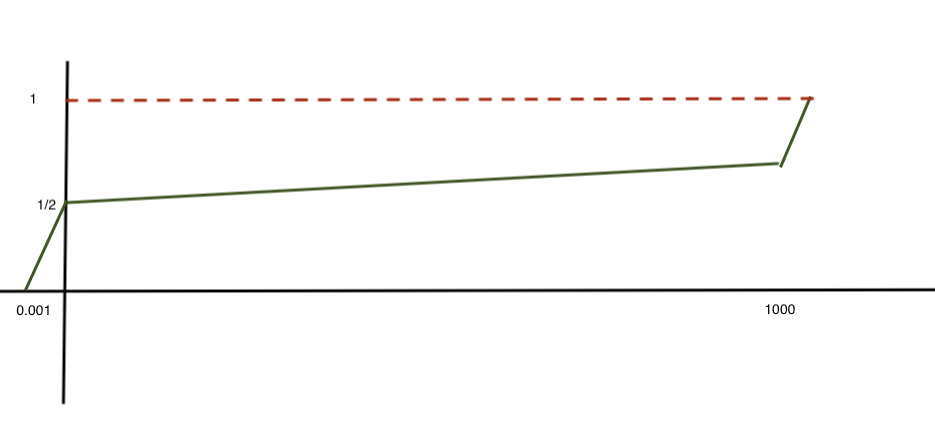
\includegraphics[width=0.5\textwidth]{/Users/kajal/Documents/statistics/resources/hw1/Figure_5.png}
	\caption{مثال نقض برای قسمت آ سوال چهار}
\end{figure}

\subproblem{}
اگر میانه توزیع را برای حالت پیوسته تعریف کنیم نقطه ای در تابع چگالی که در آن انتگرال قبل و بعد از أن برابر با یک دوم میشود این دقیقا تعریفی هست که در صورت سوال گفته شده و میانه در آن می افتد.

\subproblem{}
برای این قسمت کافیست یک توزیع نامتقارن ارایه دهیم که هر دوی میانه و میانگین عوض این مجموعه باشند.
\begin{figure}[H]
	\centering
	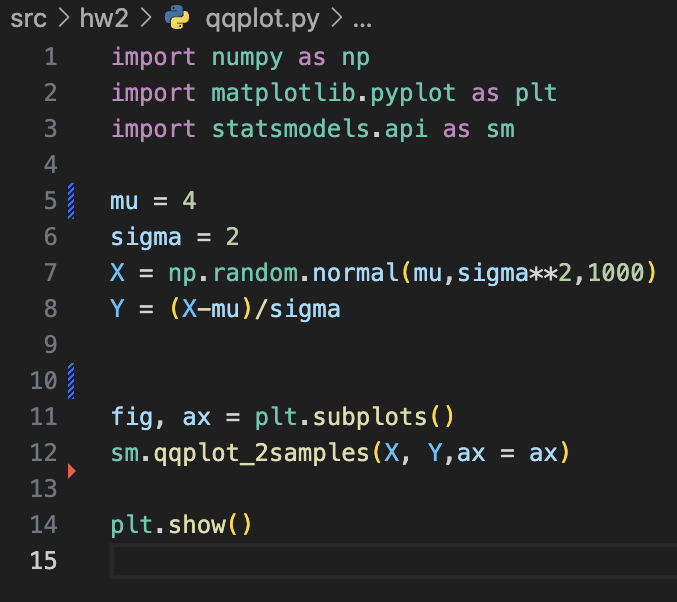
\includegraphics[width=0.5\textwidth]{/Users/kajal/Documents/statistics/resources/hw1/Figure_6.png}
\end{figure}
در شکل بالا به صورت شهودی مشخص است که میانگین و میانه هر دو در قسمت وسط نمودار می افتند و توزیع دقیقا متقارن نیست.
